\documentclass[onecolumn, draftclsnofoot,10pt, compsoc]{IEEEtran}
\usepackage{url}
\usepackage{setspace}
\usepackage{graphicx}
\usepackage{xcolor}
\usepackage{textcomp}
\usepackage{listings}
\usepackage{geometry}
\lstset{
	language=C,
	keywordstyle=\bfseries\ttfamily\color[rgb]{0,0,1},
	identifierstyle=\ttfamily,
	commentstyle=\color[rgb]{0.133,0.545,0.133},
	stringstyle=\ttfamily\color[rgb]{0.627,0.126,0.941},
	showstringspaces=false,
	basicstyle=\small,
	numberstyle=\footnotesize,
	numbers=left,
	stepnumber=1,
	numbersep=10pt,
	tabsize=8,
	breaklines=true,
	prebreak = \raisebox{0ex}[0ex][0ex]{\ensuremath{\hookleftarrow}},
	breakatwhitespace=false,
	aboveskip={1.5\baselineskip},
  columns=fixed,
  upquote=true,
  extendedchars=true
}
\renewcommand{\lstlistingname}{Code Example}

\graphicspath{ {./exPics} }
\geometry{textheight=9.5in, textwidth=7in}

% 1. Fill in these details
\def \CapstoneTeamName{     One Clock to Rule Them all}
\def \CapstoneTeamNumber{       57}
\def \GroupMemberOne{           Tasman Thenell}
\def \GroupMemberTwo{           Tristan Hari}
\def \GroupMemberThree{         Scott Metzsch}
\def \CapstoneProjectName{      One Clock to Rule Them all}
\def \CapstoneSponsorCompany{   Oregon State University}
\def \CapstoneSponsorPerson{        Dr. Victor Hsu}

% 2. Uncomment the appropriate line below so that the document type works

\def \DocType{		%Problem Statement
				%Requirements Document
				%Technology Review
				%Design Document
				Progress Report
				}



\newcommand{\NameSigPair}[1]{\par
\makebox[2.75in][r]{#1} \hfil   \makebox[3.25in]{\makebox[2.25in]{\hrulefill} \hfill        \makebox[.75in]{\hrulefill}}
\par\vspace{-12pt} \textit{\tiny\noindent
\makebox[2.75in]{} \hfil        \makebox[3.25in]{\makebox[2.25in][r]{Signature} \hfill  \makebox[.75in][r]{Date}}}}
% 3. If the document is not to be signed, uncomment the RENEWcommand below
\renewcommand{\NameSigPair}[1]{#1}

%%%%%%%%%%%%%%%%%%%%%%%%%%%%%%%%%%%%%%%
\begin{document}
\begin{titlepage}
    \pagenumbering{gobble}
    \begin{singlespace}
        %\includegraphics[height=4cm]{coe_v_spot1}
        \hfill
        % 4. If you have a logo, use this includegraphics command to put it on the coversheet.
        %\includegraphics[height=4cm]{CompanyLogo}
        \par\vspace{.2in}
        \centering
        \scshape{
            \huge CS Capstone \DocType \par
            {\large\today}\par
            \vspace{.5in}
            \textbf{\Huge\CapstoneProjectName}\par
            \vfill
            {\large Prepared for}\par
            \Huge \CapstoneSponsorCompany\par
            \vspace{5pt}
            {\Large\NameSigPair{\CapstoneSponsorPerson}\par}
            {\large Prepared by }\par
            Group\CapstoneTeamNumber\par
            % 5. comment out the line below this one if you do not wish to name your team
            %\CapstoneTeamName\par
            \vspace{5pt}
            {\Large
                \NameSigPair{\GroupMemberOne}\par
                \NameSigPair{\GroupMemberTwo}\par
                \NameSigPair{\GroupMemberThree}\par
            }
            \vspace{20pt}
        }
        \begin{abstract}
        % 6. Fill in your abstract
            The purpose of this document is to discuss the progress of the One Clock to Rule Them All project and what our team has done during the spring term.
Included is an explanation of each document updated during this period of time and a summary of the progress made during each week of the term.
In addition, this process is reflected in retrospective which discusses challenges and difficulties as well as progress.
        \end{abstract}
    \end{singlespace}
\end{titlepage}
\newpage
\pagenumbering{arabic}
\tableofcontents
% 7. uncomment this (if applicable). Consider adding a page break.
%\listoffigures
%\listoftables
\clearpage

% 8. now you write!
\section{Project Purpose and Goals}
The background of the product arises from the personal interest of our client, Victor Hsu.
While there are similar products already on the market, QWLock by Ziegert and Funk for example, these products suffer from high prices and low availability.
These items traditional occupy a designer market niche which doesn't allow most people to experience the ownership of one.
In addition to these problems, it is also difficult to track down a model that has english lettering, as Ziegert is based in Germany.

We are not the first group of people to be inspired by the unique aesthetic and function of the word clock.
There are plenty of DIY projects online that also attempt to solve the problems of price and availability.
While these projects have been a valuable source of insight for the project, they are often very complicated and considered outside the comfort level of our expected users.
The intention of this product is to improve upon the situation by making the creation of a word clock less expensive, simpler, or both.

The clock we are making will be completely self contained with a battery or wall plug being used to power the clock.
There will be a microcontroller that is used to control the LEDs on the display and interface with the RTC in order to provide accurate timekeeping capabilities.

On the side of the clock there will be 3 buttons that will be used to set the time on the clock and change features.
Each button provides a specific function depending on the software context.
An example of this system when a basic menu is being manipulated would have two buttons providing up and down scrolling and one button to select an option or submenu.

The microcontroller will be the central piece of hardware in our clock and have the software for running it embedded into it.
The RTC will be connected to the board through 6 ports and will be used to check the time periodically to verify that the time is still correct.
The LEDs will also be connected to the board and the microcontroller will send data to the LEDs that tell them which LEDs to light up.
Lastly the 4 buttons will be connected to the microcontroller to set time and access additional features added to the clock.

The clock will also provide a way for the user to set and edit alarms. While making an audible alarm wasn’t planned, user programmable alarms indicated by the display flashing are expected functionality.
Aside from that, all the other goals were simply that: it continues to operate in the normal range of temperature, at least a year straight, and is visible from 10-20 feet.


\section{Current State of project}

\subsection{Hardware}
In terms of hardware we have all of our electronic components working.
The Arduino Uno is working correctly and can communicate with the LEDs, RTC, and buttons.
The LEDs are all soldered together and have valid connections between the 12 strips.
We also have a power adapter with more amps that we are using to power both the board and LEDs.

In terms of the case hardware we are almost done with the case.
We have the 4 sides of the case cut to size with grooves cut for the front and back plate to slide in.
We have also stained these 4 sides.

\subsection{Software}
The current state of the software for the program is solid but needs more testing.
Due to difficulties relating to hardware assembly, large chunks of code have only been lightly tested.
That being said, feature completeness has been achieved and will be demonstrated during Expo.

The code is broken into two main components: the hardware abstractions and libraries, and example programs that use those libraries.
Each main hardware component (RTC, Buttons, and LEDs) are wrapped in abstractions which handle setting up these objects as well as facilitating ease of use.
Our example code is what presents the features described in our requirements to the user.

The core of the project is broken into a group of software libraries which are tied together in the main Arduino program loop.
These acts as the “operating system” of the clock from which different programs can be run, the running program can be changed, and alarms can trigger.

To get more detailed about this operating system comparison, each program for our system is a subclass of an abstract class called “state”.
All states share four common functions by which the operating system will interact with them.
The first of these functions is a constructor: a function which does any “run-once” setup for the program or state.

Three additional functions form the interface with between the operating system code and the running program: handleInput, runLogic, and drawFrame.
The first of these functions is tasked with dealing with user input.
The second function does any computing or processing work that needs to happen for the state.
The final function is tasked with updating the screen of the clock.
For some states this could be menu text, for others it could be the time in words, and for others it might be a digital time.

The second set of software written for our project is a set of example states.
These could be compared to Internet Explorer and MS Paint that come bundled with Windows.
These example states are a set of programs that run on top of the aforementioned set of abstractions which form the operating system for this product.

The example states (or programs) that are included in our project are geared towards meeting the software functionality requirements for our project.
Some of the states we have developed which will be shown off at expo are: normal word clock, digital clock, system menu, add/remove alarms, game of snake,  LED demo, and a triggered alarm.
Thanks to the high level abstraction offered by our hardware libraries, most of these states are relatively simple which was one of the goals of the project.

\subsection{Technology Review}
The technology review has been updated to reflect several changes in the project that have occured over the past two months.
The largest changes take the form of a change in the development board.
While the MPLABS Xpress board seemed like a good idea on paper, it didn't have much in the way of software support.
In addition to this, the documentation and code examples for the board were ranging from poor to nonexistant.

The new board chosen to replace it is an Arduino Uno.
This board has better software support and documentation by a very large margin.
This is documented in the Technology Review in the form of discussing the new board as well as the libraries that come with it.
Extensive research into libraries allowed development to progress more in two weeks than it had duing the six weeks prior.

\section{Remaining Work}
\subsection{Hardware}
Our remaining problem is that we are waiting for our final clock face cut from Kevin.
We should have started the prototyping process sooner to allow for more iterations of the case and clock face before we needed our final product.
Once we have the final test cut back from Kevin we will have all the hardware sections of the project completed.

\subsection{Software}
The largest remaining piece of work that needs to be done is debugging.
Various technical and cranial setbacks meant that we didn’t have a full set of the hardware assembled to test code on until somewhat recently.
Debugging is going well and is following the logical order of necessity: state manager first, display library second, time library third, and lastly button control.
That being said, all the core features are on course to be functional at Expo.

In addition to a scrolling text library, the code for static text needs to be finished.
This functionality allows the clock to show words of length four or less in fixed positions.
This was left until the end of development as scrolling text is significantly more complicated and static text can reuse most of the same code.

Another requested feature that won’t be complete for Expo is a color gradient generator.
This boils down to coming up with an algorithm that generates a unique color for the time of day.
The idea behind this capability is that the word clock (or other modes) can gradually shift through pleasant colors throughout the day.
The holdup here is an algorithm.
The function infrastructure is already in place.

Being able to change the simulated pace of time for the sake of demonstration is one feature we are rushing to complete before expo.
This will act as a wrapper around the get time functions in the clock so that we can accelerate the passage of time for the clock.
This would be useful for demonstrating alarms going off or the gradual change in color if that feature is ready by Friday.

Another item that remains on the “to-do” list is rewriting the alarm system to not rely on hardware alarms.
While using the hardware alarm feature on the Real Time Clock (RTC) can work fine, it would easier and cleaner to have alarms be handled in software.
This also frees the hardware alarms up for usage in project code without conflicting with clock functionality.
Another perk of this change would be that it makes it even simpler to port our project to a different RTC chip because we use less specific hardware features.

The last part of the project that needs to be completed before we turn our work over to our client is documentation.
Code interface has been commented to make it easy to interact with functions.
That being said, we need to produce a set of formal documentation about using our code as well as further documenting the example classes (programs) that run the basic clock functionality.
Documentation was set aside to get things ready for Expo which means it will need to be a top priority in the three remaining weeks after Expo.

\section{Impeding Factors}
Over the course of the project there were two major things that impeding progress for us.
The first of which is the original microcontroller we had.
The MPBLABXpress Evaluation board we started with looked appealing and had a nice demo example, upon further inspection we found that this was just a nice appearance.
Once we started looking into writing code to control a strip of LEDs we ran into many issues.
Large sections of the code is auto generated which made it difficult to understand and make edits to files.
Second the problem is that library integration was difficult to implement and we would be using multiple libraries to control the RTC and LEDs.
When we came to the conclusion that this board wasn’t going to work we decided to move to an Arduino Uno for our microcontroller.

The second main issue we had in our project was designing the case.
With all of us being CS students we have limited woodworking experience.
To get around this problem we created multiple prototypes and talked with people at lumber stores to learn about different techniques and wood we might use for the case.
With the multiple people and prototypes we made our final case has turned out great and has a nice finish and appearance.

\section{Code Samples}
\subsection{Scrolling Text}
\lstinputlisting[language=c++, caption=Scrolling text Example., captionpos=b]{codeExamples/demoState.cpp}
One of the key abstractions that powers the interface for the clock: scrolling text.
Our software supports two independent lines of text which can be set, cleared, and updated independently.
This was done in order to be able to show text that isn’t among the words cut into the clock faceplate.
One place this is crucial is for displaying menu text.
\vspace{5mm}
\subsection{Menu Code}
\lstinputlisting[language=c++, caption=Main Menu State., captionpos=b]{codeExamples/mainMenu.cpp}
Another core UI element in the menu.
For our system, a menu is composed of two sections: the menu title (displayed on the top row of text), and the menu options (displayed on the lower row).
Rather than having to right clusters of switch statements and other conditional logic every time a manu is needed, a menu item is provided.
This object does all the heavy lifting of displaying menus and handling user interaction.
\vspace{5mm}
\subsection{The "Operating System"}
\lstinputlisting[language=c++, caption=Core System Loop., captionpos=b]{codeExamples/clean.cpp}
Displayed above is the core code for running the clock.
A user of our software need not alter any of this, they only need to select the starting state of the clock.
The key pieces here are check for hardware signals (from buttons or RTC), run the current program, change the running program if required, and run cleanup to prepare for a new program.

\section{Project Pictures}
\centering
\includegraphics[width=0.8\textwidth, natwidth=600,natheight=800]{./exPics/scott.eps} %natwidth=3024,natheight=4032
\includegraphics[width=0.8\textwidth, natwidth=600,natheight=800]{./exPics/wood.eps}
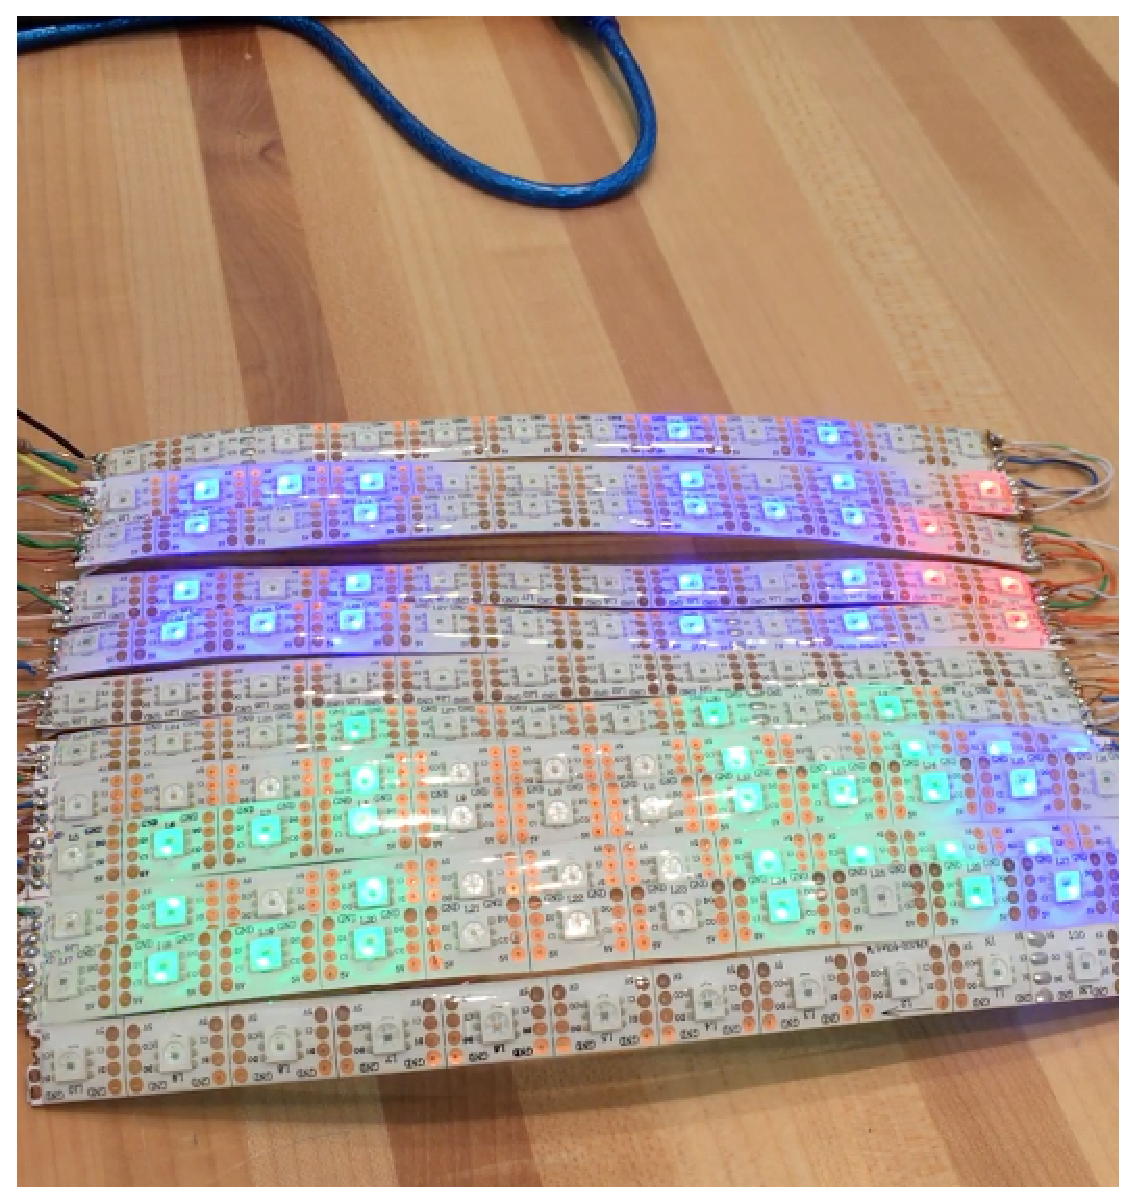
\includegraphics[width=0.8\textwidth, natwidth=529,natheight=532]{./exPics/light.eps}

\end{document}
